\begin{flushleft}
\subsection{Kildekode indholdsfortegnelse}
\subsection{Brugertests}
\begin{figure}[H] %brug begin{figure} til alle figurer.
    \centering
    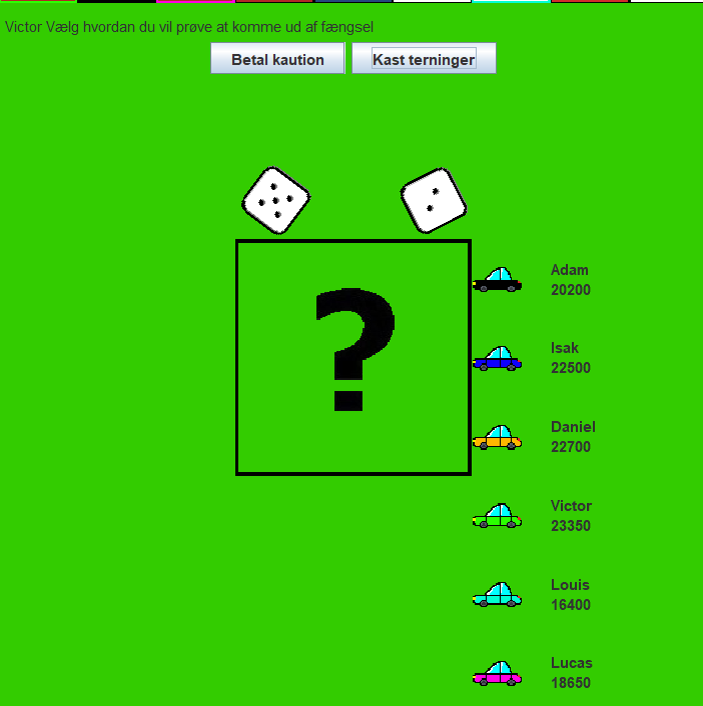
\includegraphics[width=16cm]{Report/figures/Usertests/BilagTC01.png}
    \caption{TC01 Screenshot}
    \label{TC01Bilag}
\end{figure}\begin{figure}[H] %brug begin{figure} til alle figurer.
    \centering
    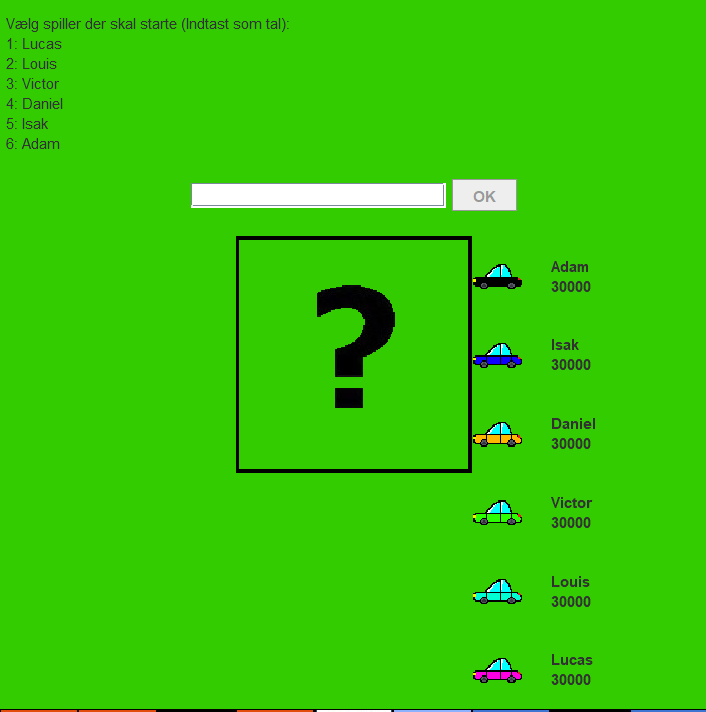
\includegraphics[width=16cm]{Report/figures/Usertests/BilagTC02.png}
    \caption{TC02 Screenshot}
    \label{TC02Bilag}
\end{figure}\begin{figure}[H] %brug begin{figure} til alle figurer.
    \centering
    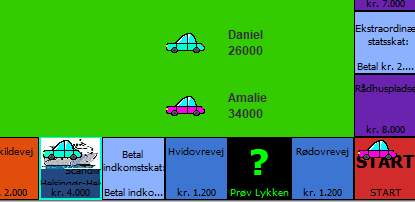
\includegraphics[width=16cm]{Report/figures/Usertests/BilagTC03.png}
    \caption{TC03 Screenshot}
    \label{TC03Bilag}
\end{figure}
\end{flushleft}

\label{endOfDoc}